% Documentation of the RibosomalFrameShift sensor

\subsubsection{\texttt{Sensor.RibosomalFrameShift}}

\paragraph{Description}

This plugins simulates ribosomal frameshifts allowing alternative translation of a mRNA sequence 
by changing the open reading frame. At each occurence of the pattern \texttt{RibosomalFrameShift\-.pat[i]} in the sequence, 
the plugin predicts a frameshift signal at the position \texttt{RibosomalFrameShi\-ft.newStatePos[i]} in the pattern.
The parameter \texttt{RibosomalFrameShift.type[i]} represents the type of frameshift and its position according to the open 
reading frame. A -1 frameshift can be seen as the deletion of the nucleotide before the position 
\texttt{RibosomalFrameShift.newStatePos[i]}, while a +1 frameshift as the insertion of a nucleotide to the position \texttt{RibosomalFrameShift.newStatePos[i]}.

Three values allow to represent a -1 frameshift in specific open reading frames:
\begin{itemize}
\item \texttt{deletion1} : deletion of the first nucleotide of the codon
\item \texttt{deletion2} : deletion of the second nucleotide of the codon
\item \texttt{deletion3} : deletion of the third nucleotide of the codon
\end{itemize}

Three values allow to represent a +1 frameshift in specific open reading frames:
\begin{itemize}
\item \texttt{insertion1} : insertion of a nucleotide before the first nucleotide of the codon
\item \texttt{insertion2} : insertion of a nucleotide before the second nucleotide of the codon
\item \texttt{insertion3} : insertion of a nucleotide before the third nucleotide of the codon
\end{itemize}

Set \texttt{RibosomalFrameShift.requiredEstSupport[i]} to 1 to only predict ribosomal frameshift if there is an EST support.

The corresponding uniform costs for using or rejecting a signal can be set using the \texttt{RibosomalFrame\-Shift.patP*[i]} 
and \texttt{RibosomalFrameShift.patPNo*[i]} parameters.


Here is an example of parameters to catch the -1 frameshift A\_AA.A\_AA.C 
(underscores separate codons in the initial frame and dots separate codons in the new -1 frame):

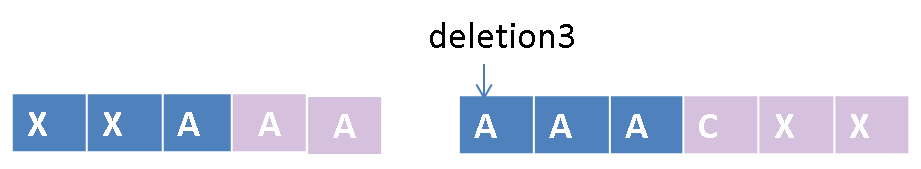
\includegraphics[width=10cm]{ExampleFS.png}

\begin{Verbatim}[fontsize=\small]
RibosomalFrameShift.type[0] deletion3 
RibosomalFrameShift.pat[0]  AAAAAAC      
RibosomalFrameShift.newStatePos[0] 4   # Position of the frameshift in the pattern
RibosomalFrameShift.patP*[0] -25
RibosomalFrameShift.patPNo*[0] 0
RibosomalFrameShift.requiredEstSupport[0] 0 # 1 if an EST support is required
#
Sensor.RibosomalFrameShift.use     1
Sensor.RibosomalFrameShift         1        # Sensor priority
\end{Verbatim}

The sensor is activated by setting the value 1 (one instance of the
plugin) or an integer (i instance) for the parameter
\texttt{Sensor.RibosomalFrameShift.use} in the parameter file.

\paragraph{Input files format}

No file input.

\paragraph{Integration of information}

All predictions that use a predicted frameshift receive the
corresponding \texttt{Ribosomal\-FrameShift.patP*[i]} penalty while those that go through
a predicted frameshift while they could have used it receive a
\texttt{RibosomalFrameShift.patPNo*[i]} penalty.

\paragraph{Post analyse}

No post analyse.

\paragraph{Graph}

No plot.
